\documentclass[tikz]{standalone}

\usepackage{amsmath}
\usepackage{lmodern}
\usepackage{pgfplots}
%\usepackage{physics}

\let\Re\undefined
\let\Im\undefined
\DeclareMathOperator{\Re}{\operatorname{Re}}
\DeclareMathOperator{\Im}{\operatorname{Im}}

\usetikzlibrary{arrows.meta}
%\pgfplotsset{compat=1.17}

\definecolor{exotic orange}{RGB}{255,128,0}
\definecolor{exotic green}{RGB}{0,102,102}
\definecolor{exotic blue}{RGB}{67,132,161}
\definecolor{exotic red}{RGB}{250,86,86}

\begin{document}
	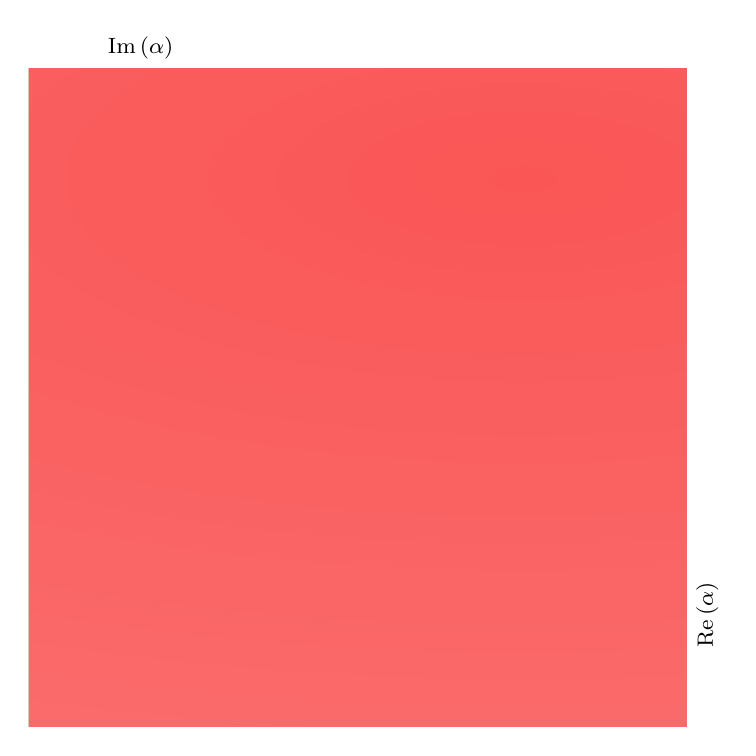
\begin{tikzpicture}[
		font=\fontsize{8}{9}\selectfont,
	]
		\begin{axis}[
			width=0.95\linewidth,
			axis lines=center,
			axis equal image,
			xlabel={$\Re\left(\alpha\right)$},
			ylabel={$\Im\left(\alpha\right)$},
			ticks=none,
			xmin=-.2,
			xmax=+1,
			ymin=-.2,
			ymax=+1,
			domain=-180:180,
			samples=100,
			axis line style={thick},
			x label style={
				at={(axis description cs:1,0.17)},
				anchor=north,
				rotate=90,
			},
			y label style={
				at={(axis description cs:0.17,1)},
				anchor=south,
			},
		]
			\shadedraw[inner color=exotic blue, outer color=exotic blue!40, draw=none] (axis cs:0.8,0.8) circle (10);
			\shadedraw[inner color=exotic orange, outer color=exotic orange!40, draw=none] (axis cs:0.0,0.0) ellipse (15 and 7);
			\shadedraw[inner color=exotic green, outer color=exotic green!40, draw=none] (axis cs:0.0,0.0) ellipse (13 and 5);
			\draw[-Latex, gray, thick] (axis cs:0.65,0.75) -- (axis cs:0.1,0.1) node[midway, fill=white]{Channel};
			\draw[-Latex, gray, thick] (axis cs:0.8,0.94) -- (axis cs:0.7,0.94) node[above, midway]{Cloning};
			\shadedraw[inner color=exotic red, outer color=exotic red!40, draw=none] (axis cs:0.7,0.8) ellipse (13 and 5);
		\end{axis}
	\end{tikzpicture}
\end{document}